\documentclass[sigchi-a, authorversion,table]{acmart}
\usepackage{booktabs} % For formal tables
\usepackage{ccicons}  % For Creative Commons citation icons
\usepackage{tabularx}
\usepackage{multirow}
\usepackage{multicol}
\usepackage{xcolor}
\usepackage{dcolumn}
\usepackage{url}
\newcolumntype{d}[1]{D{.}{.}{#1}}
\usepackage[capitalise,nameinlink,noabbrev]{cleveref}                 
\usepackage[colorinlistoftodos]{todonotes}
%\setlength{\marginparwidth}{2,5cm}

%Cleverref works using this
\setcounter{secnumdepth}{2}

% Copyright
\setcopyright{none}
%\setcopyright{acmcopyright}
%\setcopyright{acmlicensed}
%\setcopyright{rightsretained}
%\setcopyright{usgov}
%\setcopyright{usgovmixed}
%\setcopyright{cagov}
%\setcopyright{cagovmixed}


% DOI
\acmDOI{}

% ISBN
%\acmISBN{123-4567-24-567/08/06}

%Conference
\acmConference[FIS'18]{Fachpraktikum Interaktive Systeme}{July 2018}{Stuttgart, Germany}
\acmYear{2018}
\copyrightyear{2018}

\acmPrice{1000.00}

%\acmBadgeL[http://ctuning.org/ae/ppopp2016.html]{ae-logo}
%\acmBadgeR[http://ctuning.org/ae/ppopp2016.html]{ae-logo}

\begin{document}
\title{Simple Touch Prediction with Built-In IMUs}

\author{Benedict Steuerlein}
\affiliation{%
  \institution{University of Stuttgart}
  \city{Stuttgart}
  \country{Germany} }
\email{st111340@stud.uni-stuttgart.de}

\author{Felix Bühler}
\affiliation{%
  \institution{University of Stuttgart}
  \city{Stuttgart}
  \country{Germany} }
\email{st117123@stud.uni-stuttgart.de}


% The default list of authors is too long for headers.
\renewcommand{\shortauthors}{F. Author et al.}


%
% The code below should be generated by the tool at
% http://dl.acm.org/ccs.cfm
% Please copy and paste the code instead of the example below.
%


\begin{CCSXML}
<ccs2012>
 <concept>
<concept_id>10003120.10003121.10003122.10003334</concept_id>
<concept_desc>Human-centered computing~User studies</concept_desc>
<concept_significance>500</concept_significance>
</concept>
<concept>
<concept_id>10003120.10003138.10003141</concept_id>
<concept_desc>Human-centered computing~Ubiquitous and mobile devices</concept_desc>
<concept_significance>500</concept_significance>
</concept>
</ccs2012>
\end{CCSXML}

\ccsdesc[500]{Human-centered computing~User studies}
\ccsdesc[500]{Human-centered computing~Ubiquitous and mobile devices}
\begin{abstract}
Lorem ipsum dolor sit amet, consectetuer adipiscing elit. Aenean commodo ligula eget dolor. Aenean massa. Cum sociis natoque penatibus et magnis dis parturient montes, nascetur ridiculus mus. Donec quam felis, ultricies nec, pellentesque eu, pretium quis, sem. Nulla consequat massa quis enim. Donec pede justo, fringilla vel, aliquet nec, vulputate eget, arcu. In enim justo, rhoncus ut, imperdiet a, venenatis vitae, justo. Nullam dictum felis eu pede mollis pretium. Integer tincidunt. Cras dapibus. Vivamus elementum semper nisi. Aenean vulputate eleifend tellus. Aenean leo ligula, porttitor eu, consequat vitae, eleifend ac, enim. Aliquam lorem ante, dapibus in, viverra quis, feugiat a, tellus. Phasellus viverra nulla ut metus varius laoreet. Quisque rutrum. Aenean imperdiet. Etiam ultricies nisi vel augue. Curabitur ullamcorper ultricies nisi. Nam eget dui. Etiam rhoncus. Maecenas tempus, tellus eget condimentum rhoncus, sem quam semper libero, sit amet adipiscing sem neque sed ipsum. Nam quam nunc, blandit vel, luctus pulvinar
%See: \url{https://users.ece.cmu.edu/~koopman/essays/abstract.html}
\todo{noch ein bis zwei doofe keywords finden}
\end{abstract}


\keywords{Touch prediction; Smartphone; sensors; regression; deep learning; .}

\maketitle



\graphicspath{{./pictures/}}
\section{Introduction}
Touch is the preferred input method on smartphones today. 
Current research and manufacturers are constantly trying to improve and enhance the interaction on smartphones. 
One way can be the extension of interactable space with interaction possibilities on the devices' backside \cite{BACHELORARBEIT}.
Another way to extend interaction is the introduction of additional touch gestures on the touchscreen \cite{PALM TOUCH}.
In this paper we present a machine learning model for touch prediction on smartphones using only the phones' built-in inertial measurement units (IMU).




\section{Related Work}

Motivate your project by reporting about related work and common goals.
\section{Data Collection Study}

We conducted a data collection study to gather IMU data while performing touches on a smartphone.
Our collected data set consists of 6 smartphone sensors that were sampled while participants performed successive touches on the smartphones front side. 
For our data collection study we used a repeated-measures design with one independent variable: \textsc{phone}, which was counterbalanced using Latin Balanced squares. 
The total amount of conditions was: \textsc{phone} $ = 4$.

\subsection{Apparatus}
\begin{margintable}
	\vspace{-3.9cm}
	\centering
	\begin{tabularx}{1.03\marginparwidth}{Xd{2.1}d{2.1}d{1.1}}
		\toprule
		\multicolumn{1}{l}{\multirow{3}{*}{\shortstack[c]{\textbf{Device}}}}&
		\multicolumn{1}{c}{\multirow{3}{*}{\shortstack[c]{\textbf{Release}}}}&    
		\multicolumn{1}{c}{\multirow{3}{*}{\shortstack[c]{\textbf{Weight}\\ \textbf{(g)}}}} &
		\multicolumn{1}{c}{\multirow{3}{*}{\shortstack[c]{\textbf{Screen}\\ \textbf{Diagonal}\\ \textbf{(in)}}}} \\
		\\
		\\
		\midrule
		%                year   weight diag  
		S3 Mini  		& 2012 & 113 &  4. \\
		S4 				& 2013 & 130 &5.   \\
		Nexus 5X 		& 2015 & 136 &5.2  \\
		Nexus 6 		& 2014 & 184 & 6.  \\ 
		
		
		\bottomrule
		
		%	\multicolumn{1}{l}{\multirow{3}{*}{\shortstack[c]{\textbf{Device}}}}&
		&\multicolumn{1}{c}{\multirow{3}{*}{\shortstack[c]{\textbf{Height}\\ \textbf{(cm)}}}} &
		\multicolumn{1}{c}{\multirow{3}{*}{\shortstack[c]{\textbf{Width}\\ \textbf{(cm)}}}} &
		\multicolumn{1}{c}{\multirow{3}{*}{\shortstack[c]{\textbf{Depth}}}} \\ 
		\\
		\\
		\midrule
		%		          height  width  depth
		S3 Mini  		& 12.16 & 6.3  & 0.99 \\
		S4 				& 13.7  & 7.0  & 0.79 \\
		Nexus 5X 		& 14.7  & 7.26 & 0.79 \\
		Nexus 6 		& 15.93 & 8.3  & 1.01 \\
		
		\bottomrule
	\end{tabularx}%
	\caption[Smartphone data]{\small Data about the smartphones that were used in the study.}
	\label{tab:devices}
\end{margintable}
\begin{margintable}
	%	\vspace{-5cm}
	\centering
	\begin{tabularx}{1\marginparwidth}{Xd{2.1}d{2.1}d{1.1}d{1.1}}
		\toprule
		&
		\multicolumn{1}{c}{\multirow{2}{*}{\shortstack[c]{\textbf{S3M} \\ \textbf{0ms}}}}&    
		\multicolumn{1}{c}{\multirow{2}{*}{\shortstack[c]{\textbf{S4}\\ \textbf{0ms}}}} &
		\multicolumn{1}{c}{\multirow{2}{*}{\shortstack[c]{\textbf{N5X}\\ \textbf{0ms}}}} &
		\multicolumn{1}{c}{\multirow{2}{*}{\shortstack[c]{\textbf{N6}\\ \textbf{0ms}}}} \\
		\\
		\midrule
		%                	 Touch  33ms  66ms  
		RF & 28.11 & 34.76 &36.38 & 41.4 \\ \cmidrule{1-5}
		DT & 28.81 & 35.58 &37.03 & 42.56 \\ \cmidrule{1-5}
		KNN& 28.67 & 34.61 &36.36 & 42.91 \\ \cmidrule{1-5}
		GP & 53.35 & 66.83 &69.53 & 79.06 \\ \midrule
		
		%		\multicolumn{1}{l}{\multirow{2}{*}{\shortstack[c]{\textbf{Regressor}}}}&
		&\multicolumn{1}{c}{\multirow{2}{*}{\shortstack[c]{\textbf{S3M} \\ \textbf{33ms}}}}&    
		\multicolumn{1}{c}{\multirow{2}{*}{\shortstack[c]{\textbf{S4}\\ \textbf{33ms}}}} &
		\multicolumn{1}{c}{\multirow{2}{*}{\shortstack[c]{\textbf{N5X}\\ \textbf{33ms}}}} &
		\multicolumn{1}{c}{\multirow{2}{*}{\shortstack[c]{\textbf{N6}\\ \textbf{33ms}}}} \\
		\\
		\midrule
		%                	 Touch  33ms  66ms  
		%                	 Touch  33ms  66ms  
		RF & 27.91 & 34.29  & 36.05  & 40.45 \\ \cmidrule{1-5}
		DT & 28.39 & 35.1   & 35.03  & 41.52 \\ \cmidrule{1-5}
		KNN& 28.41 & 34.31  & 35.92  & 42.13 \\ \cmidrule{1-5}
		GP & 52.89 & 66.82  & 69.52  & 79.05 \\ 
		\midrule
		%		\multicolumn{1}{l}{\multirow{2}{*}{\shortstack[c]{\textbf{Regressor}}}}&
		&\multicolumn{1}{c}{\multirow{2}{*}{\shortstack[c]{\textbf{S3M}  \\ \textbf{66ms}}}}&    
		\multicolumn{1}{c}{\multirow{2}{*}{\shortstack[c]{\textbf{S4} \\ \textbf{66ms}}}} &
		\multicolumn{1}{c}{\multirow{2}{*}{\shortstack[c]{\textbf{N5X} \\ \textbf{66ms}}}} &
		\multicolumn{1}{c}{\multirow{2}{*}{\shortstack[c]{\textbf{N6} \\ \textbf{66ms}}}}\\
		\\
		\midrule
		%                	 Touch  33ms  66ms  
		RF &27.54 & 33.58  & 35.24  & 40.18 \\ \cmidrule{1-5}
		DT &27.9  & 32.74  & 34.67  & 39.54 \\ \cmidrule{1-5}
		KNN&28.1  & 33.99  & 35.93  & 41.62 \\ \cmidrule{1-5}
		GP &44.65 & 64.83  & 67.88  & 76.18 \\ 
		\bottomrule
	\end{tabularx}%
	\caption[Baseline data]{\small Average euclidean distances (mm) for baseline regressors.}
	\label{tab:baseline}
\end{margintable}

Our dataset was generated using four different sized smartphones on which participants had to perform a certain amount of touches (for further information see \cref{sec:tasks}).
The phones we used were a Samsung S3 Mini, a Samsung S4, a Google Nexus 5X, and a Motorola Nexus 6.
For more technical details about the used devices see \cref{tab:devices}.
Our used phone sizes range from $ 4^{\prime\prime} $ (S3) to $ 6^{\prime\prime} $ (N6). 
Using phones of these sizes we were able to cover the sizes of everyday smartphones, including some high-end devices and create a generalizable machine-learning model.



\subsection{Tasks}
\label{sec:tasks}

%\begin{marginfigure}
%	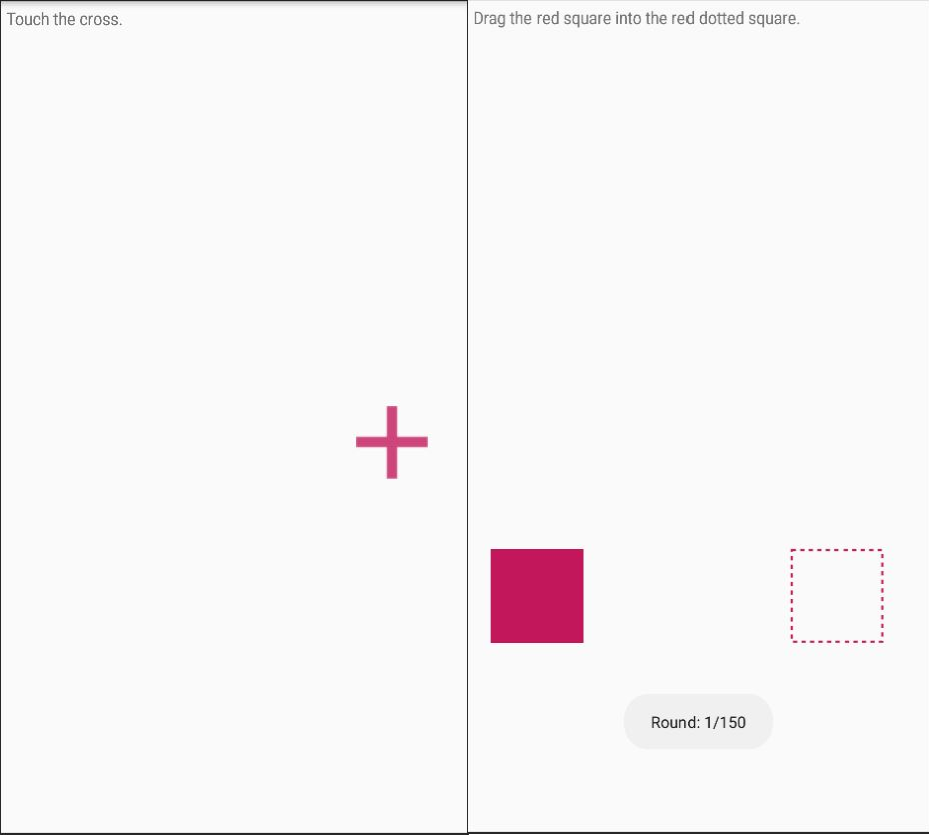
\includegraphics[width=\marginparwidth]{scur}
%	\caption{SCUR.}
%	\label{fig:tasks}
%\end{marginfigure}



For our data collection study participants had to touch points displayed as crosses in a 16 $ \times $ 9 grid on the touchscreen (see \cref{fig:touchtask}). 
%We aligned the touch points displayed as crosses in a 16 $ \times $ 9 grid. 
To achieve a high variance, we randomized the positions of the crosses within all the cells.
To avoid sequential effects, we randomized the order in which the crosses were displayed.
There were a total of 3 repetitions, resulting in a total  of $ 16 \times 9 \times 3 = 432 $ touches on one device.

Between two touches our study participants had to perform a simple \textit{Fitts' Law task} (see \cref{fig:fittstask}). 
Here participants had to drag a filled rectangle into a dashed contour of a rectangle.
This task was mainly implemented to reset the participants grip to the bottom half of the device.
Because a previous shifted grip of the hand to the upper half of the phone influences the recorded sensor data when reaching for the next target in the lower half and vice versa.
\subsection{Procedure}
Participants were either invited within the course \textit{FIS'18} or orally.
All appointments were discussed orally.
After participants have arrived they signed a consent form, and we continued measuring their hand length.
We asked the participants to take a seat on a chair without armrests and explained the study procedure and its sense.
We started carrying out the study and handed out the first phone accordingly to the balanced Latin Square order. 
After participants finished the tasks (see \cref{sec:tasks}) on the first phone, we asked them if they need a short recovery break and then continued with the next phones.
Additionally, we allowed participants to rest and put away the phone during the \textit{Fitt's Law task} because we specifically deal with this task in our preprocessing step (see \cref{sec:prepro}).
The study duration was 54 minutes on average.

\subsection{Participants}
%Some sentences are copied from Beens BA, is this sufficient? ASK SVEN OR HUY
We invited 20 right-handed fellow students as participants (15 male, 5 female).
Their age ranged between 21 and 27 ($ M=24.25$ , $SD=1.58 $). 
We measured the hand length of participants. 
The size was measured from the tip of the middle finger to the wrist crease with fingers stretched out.
Hand lengths ranged from $16.0cm$ to $21.3cm$ ($M=19.3cm$ , $SD=1.47cm$).
Our measured data covers samples from the 5th and 95th percentile of the anthropometric data reported in previous work \cite{Poston}.  

\section{Results}

\begin{margintable}
	\vspace{-4.73cm}
	\centering
	\begin{tabularx}{1\marginparwidth}{XXd{2.2}d{2.2}d{2.2}}
		
		\toprule
		
		\textbf{Model}&\textbf{Phone}&\multicolumn{1}{c}{\textbf{0ms}}&\multicolumn{1}{c}{\textbf{33ms}}&\multicolumn{1}{c}{\textbf{66ms}} \\
		\midrule
		
		\multirow{8}{*}{\textsc{single}}   &\multirow{2}{*}{\textbf{S3}}  &12.50&13.17&14.40       \\
		&                              &(7.36)&(7.82)&(8.24)       \\
		\cmidrule(r){2-5}		
		&\multirow{2}{*}{\textbf{S4}}  &17.25&18.77&19.41       \\
		&                              &(9.94)&(10.76)&(10.78)       \\
		\cmidrule(r){2-5}						 				   
		&\multirow{2}{*}{\textbf{N5X}} &17.01&18.09&19.96       \\
		&                              &(9.76)&(10.39)&(10.93)       \\
		\cmidrule(r){2-5}										   
		&\multirow{2}{*}{\textbf{N6}}  &18.87&19.78&21.52       \\
		&                              &(11.40)&(12.15)&(12.70)       \\	
		
		\midrule
		
		\multirow{8}{*}{\textsc{general}} &\multirow{2}{*}{\textbf{S3}}   &12.95&13.48&14.52        \\
		&                               &(7.57)&(7.92)&(8.38)        \\ 
		\cmidrule(r){2-5}
		&\multirow{2}{*}{\textbf{S4}}   &16.79&17.69&18.70        \\
		&                               &(10.61)&(10.99)&(11.21)        \\
		\cmidrule(r){2-5}
		&\multirow{2}{*}{\textbf{N5X}}  &17.39&17.69&18.70        \\
		&                               &(10.61)&(10.99)&(11.21)        \\
		\cmidrule(r){2-5}									      
		&\multirow{2}{*}{\textbf{N6}}   &17.53&17.75&19.53        \\ 
		&                               &(11.59)&(11.94)&(12.72)       \\									         		
		\bottomrule    
	\end{tabularx}%
	\caption[Model results]{\small Average test euclidean distances (mm) and standard deviations (brackets) for single and general models for all configurations.}
	\label{tab:results}
\end{margintable}

\subsection{Data Set \& Preprocessing}
\label{sec:prepro}
Look at \cref{tab:baseline}
We recorded a total of 1079 minutes of sensor data from the \textit{touch} and \textit{Fitt's Law task} task. 
%Since we are only interested in sensor changes during the process of reaching for a target and touching it and the purpose of the \textit{Fitt's Law task} was only for reseting the participants grip to the lower half of the phone our first step in our preprocessing pipeline was \texttt{cutting} out the sensor fragments of the \textit{Fitt's Law task}.
Due to the high sampling rate of the sensors we first removed occurring duplicates by keeping the last sensor value and timestamp.
We then up-sampled the sensors to 333.33 Hz, resulting in 1 sample given every 3ms. 
Finally, we saved 100 samples before each touch resulting in a total of 3.456.000 samples.

Up-sampling the sensors to 1 sample every 3ms resulted in a discontinuous function for each sensor axis. 
We have therefore tried applying several smoothing procedures, including a Butterworth lowpass-filter and a moving average filter.
Both approaches, however, did not lead to an increase in accuracy, so we have adhered to the unsmoothed data of the sensors.

\subsection{Baseline}
We explored basic regressors from scikit-learn \footnote{\url{https://scikit-learn.org/stable/supervised\_learning.html\#supervised-learning}} as a baseline to test whether using novel machine learning techniques is sufficient for touch prediction with IMU.
The used regressors are abbreviated as follows: RandomForestRegressor (RF), Decision Tree Regressor (DT), K Nearest Neighbors Regressor (KNN), and Gaussian Processes Regressor (GP).
We performed a grid search for the different regressors to find the best hyperparameters for each regressor.
The results for all phones with different time configurations of all regressors can be seen in \cref{tab:baseline}.

\subsection{Neural Network Structure}
We implemented a CNN using \textit{Keras} 2.2.4 based on the TensorFlow backend. 
We trained two model types, one which we call \textit{single} and one which we call\textit{general} model.
Single models were trained on sensor and touch data of single phones; general models were trained on sensor data and normalized touch data of all phones.
The model structures differs for single and general models.
Due to place restrictions 



%\footnote{\url{https://05.jupyter.interactionlab.io/user/beneste/tree/fapra-imu}}

\begin{marginfigure}
	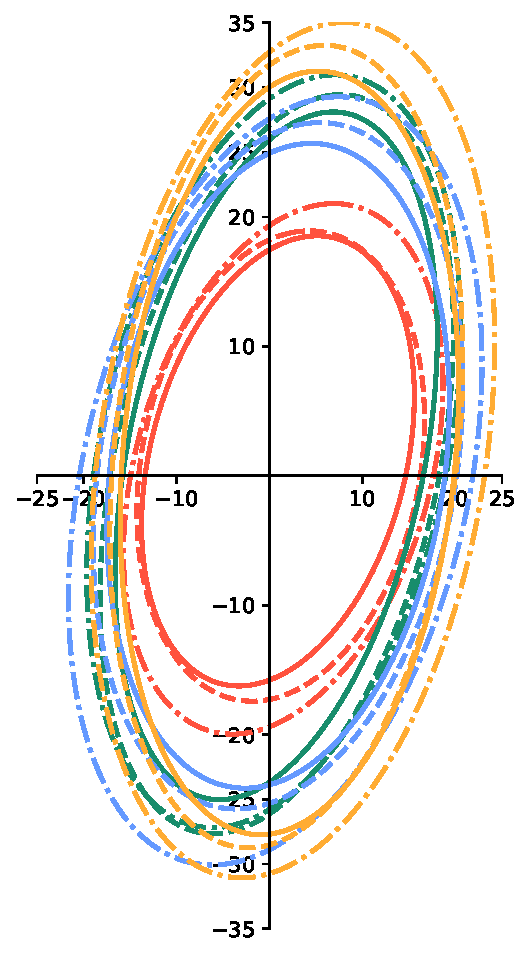
\includegraphics[height=\linewidth]{ellipses_single}
	\caption{Ellipses plot for single models.\newline}
	\label{fig:ell_single}
\end{marginfigure}

\begin{marginfigure}
	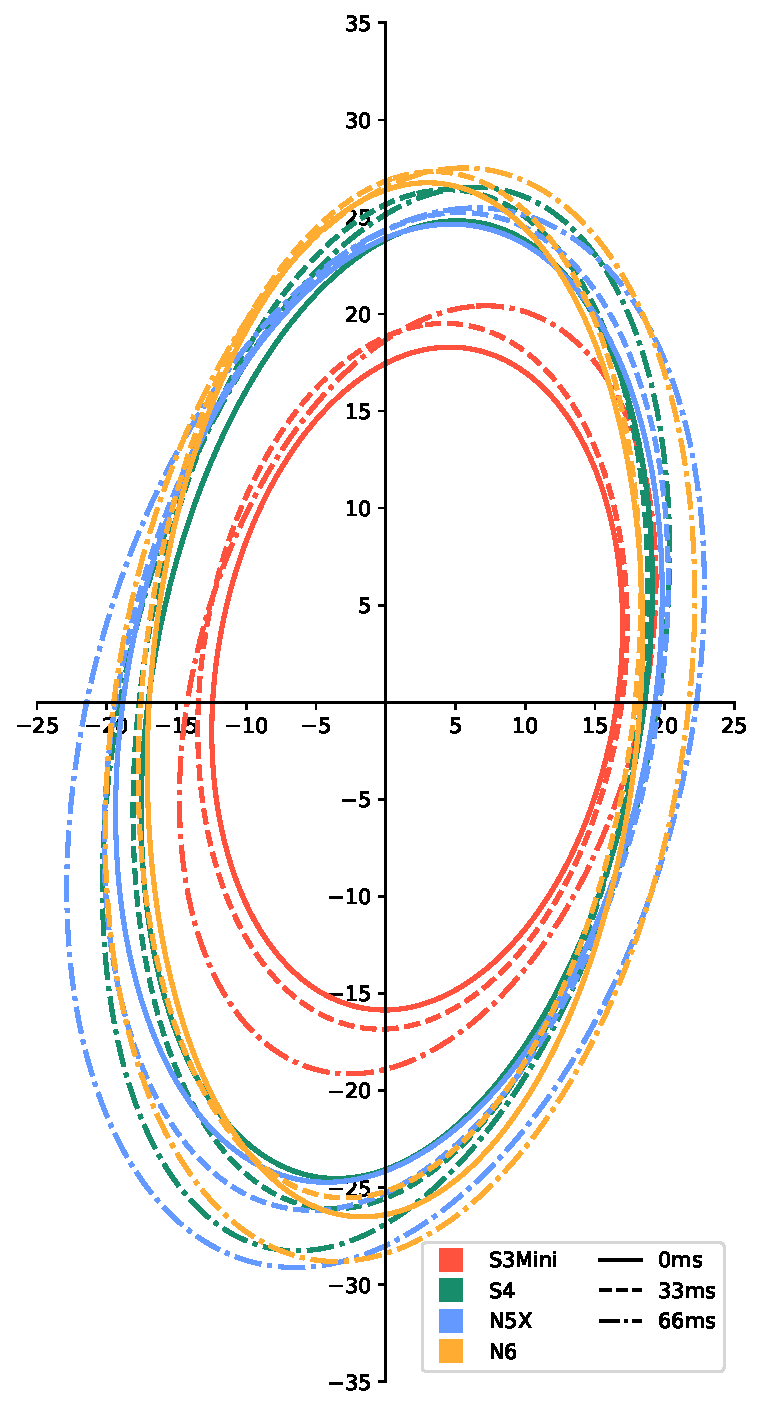
\includegraphics[height=\linewidth]{ellipses_general}
	\caption{Ellipses plot for general models.}
	\label{fig:ell_general}
\end{marginfigure}

%Report about your model. No source code!
%
%Report about the validation dataset / validation study. 
\section{Discussion}
Disuses why it is still not awesome and how this could be improved. Why this is still awesome? Think about: Nobody has done this before. 

\subsection*{Limitations}
In this paper we focused on one specific use task where users touched randomized targets on smartphones while sitting in on a chair without armrests. 
The sensor samples generated during our study are specific for this use case and thereby do not cover ordinary smartphone usage and implied phone movement when for example walking or operating the phone in a train.
\todo{Limitations of using our machine learning approach}
\section{Conclusion}
Two sentences wrap up what you have done. Than report what you achieved. 


% \begin{sidebar}
%  \textbf{Good Utilization of the Side Bar}
%
%  \textbf{Preparation:} Do not change the margin
%  dimensions and do not flow the margin text to the
%  next page.
%
%  \textbf{Materials:} The margin box must not intrude
%  or overflow into the header or the footer, or the gutter space
%  between the margin paragraph and the main left column.
%
%  \textbf{Images \& Figures:} Practically anything
%  can be put in the margin if it fits. Use the
%  \texttt{{\textbackslash}marginparwidth} constant to set the
%  width of the figure, table, minipage, or whatever you are trying
%  to fit in this skinny space.
%
%  \caption{This is the optional caption}
%  \label{bar:sidebar}
%\end{sidebar}
%
%
%
%\begin{marginfigure}
%    %\includegraphics[width=\marginparwidth]{cats}
%    \caption{In this image, the cats are tessellated within a square
%      frame. Images should also have captions and be within the
%      boundaries of the sidebar on page~\pageref{bar:sidebar}. Photo:
%      \cczero~jofish on Flickr.}
%    \label{fig:marginfig}
%\end{marginfigure}
%
%\begin{margintable}
%    \caption{A simple narrow table in the left margin
%      space.}
%    \label{tab:table2}
%    \begin{tabular}{r r l}
%      & {\small \textbf{First}}
%      & {\small \textbf{Location}} \\
%      \toprule
%      Child & 22.5 & Melbourne \\
%      Adult & 22.0 & Bogot\'a \\
%      \midrule
%      Gene & 22.0 & Palo Alto \\
%      John & 34.5 & Minneapolis \\
%      \bottomrule
%    \end{tabular}
%\end{margintable}
\newpage
\bibliography{bibliography}
\bibliographystyle{ACM-Reference-Format}

\end{document}
